\documentclass{beamer}
\usepackage{amssymb,amsfonts,color,graphicx,amsmath,enumerate,mathtools}
\usepackage{tikz} %This package offers the ability to draw pictures
\usepackage{amsthm}
\usepackage{hyperref}
\usepackage{lmodern}
\usepackage{subfig}


\theoremstyle{plain}
\newtheorem{claim}[theorem]{Claim}
\newtheorem{proposition}[theorem]{Proposition}
\newtheorem{observation}[theorem]{Observation}
\newtheorem{conjecture}[theorem]{Conjecture}
\newtheorem{remark}[theorem]{Remark}
\newtheorem{property}[theorem]{Property}
\newtheorem{exercise}[theorem]{Exercise}
\newtheorem{exercises}[theorem]{Exercises}
\newtheorem{question}[theorem]{Question}
\newcommand{\Bin}{\ensuremath{\textrm{Bin}}}
\newcommand{\Bern}{\text{Bern}}


\newcommand{\naturals}{\mathbb{N}}
\newcommand{\Z}{\mathbb{Z}}
\newcommand{\C}{\mathbb{C}}
\newcommand{\reals}{\mathbb{R}}
\newcommand{\exreals}{\overline{\mathbb{R}}}
\newcommand{\mcal}[1]{\mathcal{#1}}
\newcommand{\mable}{measurable}
\newcommand{\quats}{\mathbb{H}}
\newcommand{\rationals}{\mathbb{Q}}
\newcommand{\norm}{\trianglelefteq}
\newcommand{\Aut}{\text{Aut}}
\newcommand{\disk}{\mathbb{D}}
\newcommand{\halfplane}{\mathbb{H}}
\newcommand{\Lp}[2]{\left\|{#1}\right\|_{L^{#2}}}
\newcommand{\supp}[1]{\text{supp}({#1})}
\newcommand{\Hom}[2]{\text{Hom}_{{#1}}({#2})}
\newcommand{\tr}{\text{tr}}
\newcommand{\field}[1]{\mathbb{F}_{{#1}}}
\newcommand{\Gal}[1]{\text{Gal}\left({#1}\right)}
\newcommand{\esssup}{\text{ess sup }}
\newcommand{\essinf}{\text{ess inf }}
\newcommand{\affine}{\mathbb{A}}
\newcommand{\E}{\mathbb{E}}
\newcommand{\Var}{\text{Var}}


\title{Problems in Extremal Graph and Hypergraph Theory}
\author{Liam Hardiman}
\date{December 10, 2020}

\usetheme{Frankfurt}
%\usecolortheme{magpie}

\AtBeginSection[]{
	\begin{frame}<beamer>
		\tableofcontents[currentsection]
	\end{frame}
}

\addtobeamertemplate{navigation symbols}{}{%
    \usebeamerfont{footline}%
    \usebeamercolor[fg]{footline}%
    \hspace{1em}%
    \insertframenumber/\inserttotalframenumber
}

\begin{document}

\maketitle

% ways to think about graph substructures
%	turan-type theorems: how many edges do you need to force your substructure?
%		triangle: mantel's theorem
%		K_k: turan's theorem	


\section{Graph substructures}

	\begin{frame}{Basic Definitions}
		\begin{itemize}
			\item A \textbf{graph} $G = (V, E)$ consists of a (finite for us) set of \textbf{vertices} $V$ and a set $E$ of edges where $E\subseteq \binom{V}{2}$.

			\pause

			\item The number of vertices incident to $v\in V$ is its \textbf{degree}, $d_G(v)$.
			We let $\Delta(G)$ and $\delta(G)$ denote the maximum and minimum degree, respectively.

			\pause

			\item $H = (V', E')$ is a \textbf{subgraph} of $G$ if $V'\subseteq V$, $E'\subseteq E$ and each edge in $E'$ has both ends in $V'$.

			\pause

			%%\item $H = (V', E')$ is a \textbf{spanning subgraph} of $G = (V, E)$ if $V' = V$.\pause

			\item If $X\subseteq V$, then the \textbf{subgraph induced by $X$}, $G[X]$, is the graph with vertex set $X$ and all edges from $E$ that have both ends in $X$.


			%\item The \textbf{degree} of a vertex $v$, denoted $d_G(v)$, is the number of edges of $G$ that $v$ appears in. We let $\delta(G)$ denote the minimum degree of any of $G$'s vertices and $\Delta(G)$ the maximum.
		\end{itemize}
	\end{frame}


	\begin{frame}{Example}
		\begin{figure}
			\begin{overprint}
				\onslide<1>\centering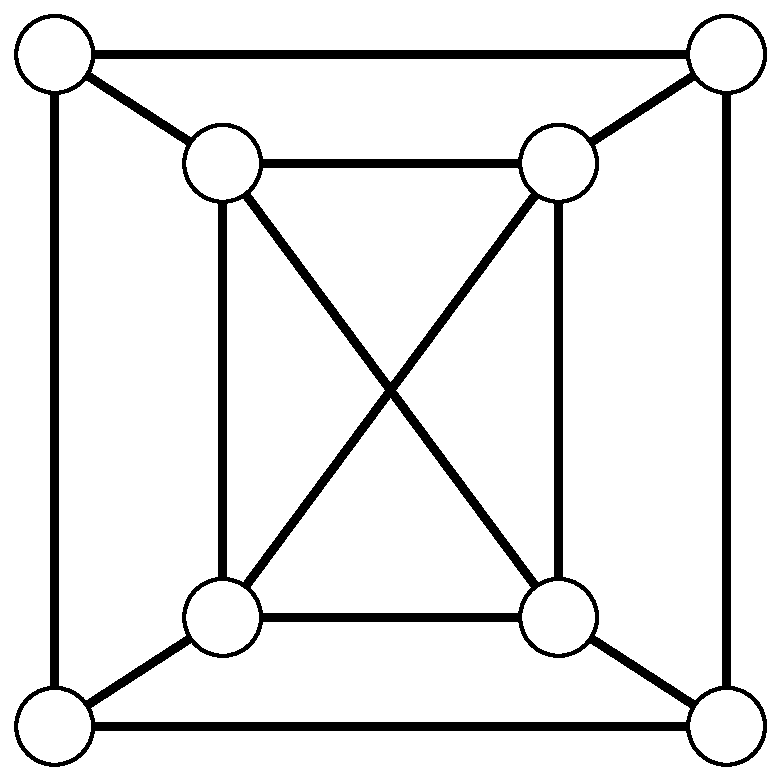
\includegraphics[scale=.5]{graph.pdf}\caption{A graph}
				\onslide<2>\centering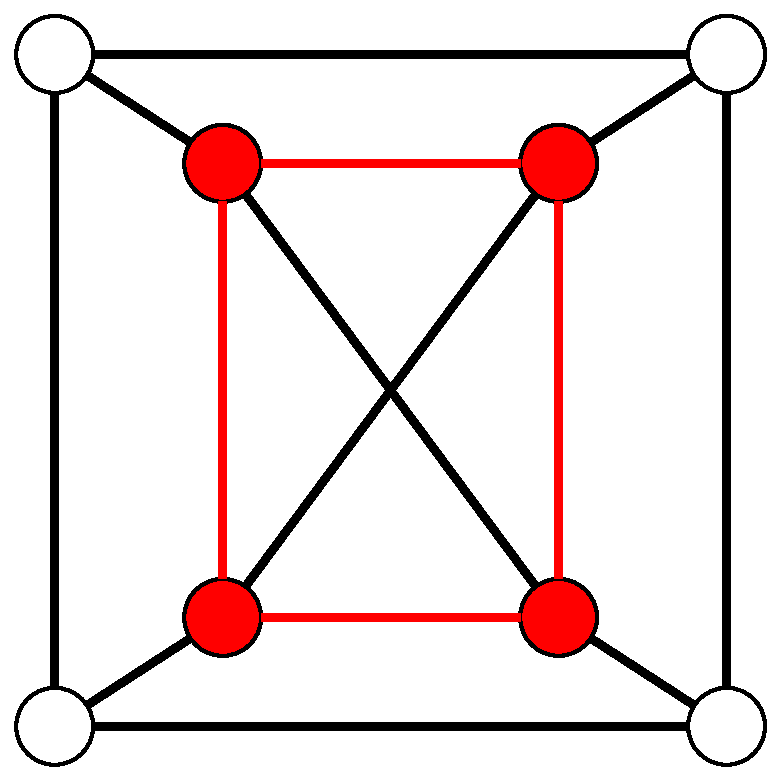
\includegraphics[scale=.5]{subgraph.pdf}\caption{A subgraph}
				\onslide<3>\centering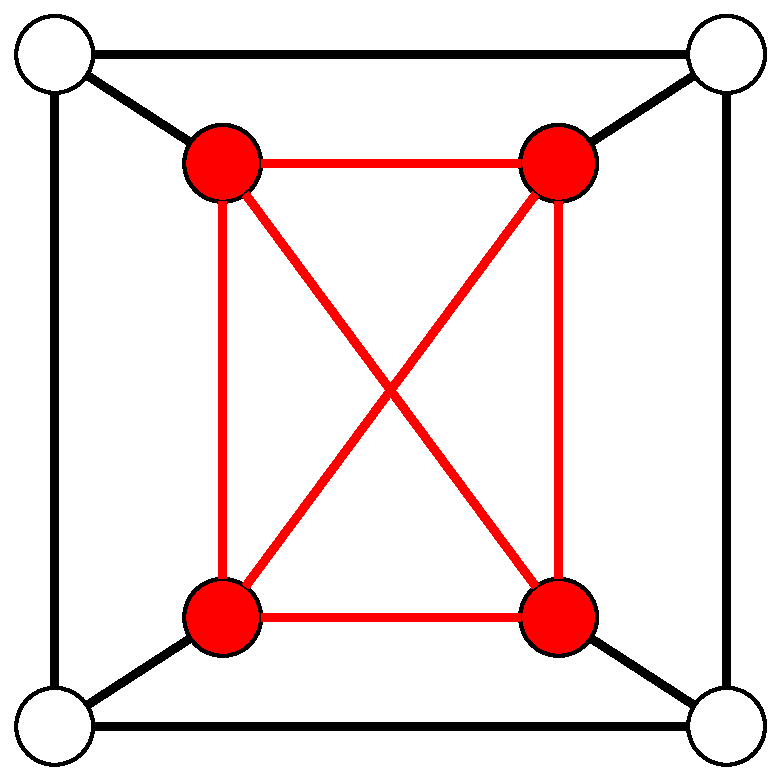
\includegraphics[scale=.5]{induced_subgraph.pdf}\caption{An induced subgraph}
			\end{overprint}
		\end{figure}
	\end{frame}


	\begin{frame}{An existence question}
		\begin{question}
			How many edges does a graph on $n$ vertices need in order to guarantee that it contains a triangle?
		\end{question}

		\pause

		\begin{figure}
			\centering
			\subfloat{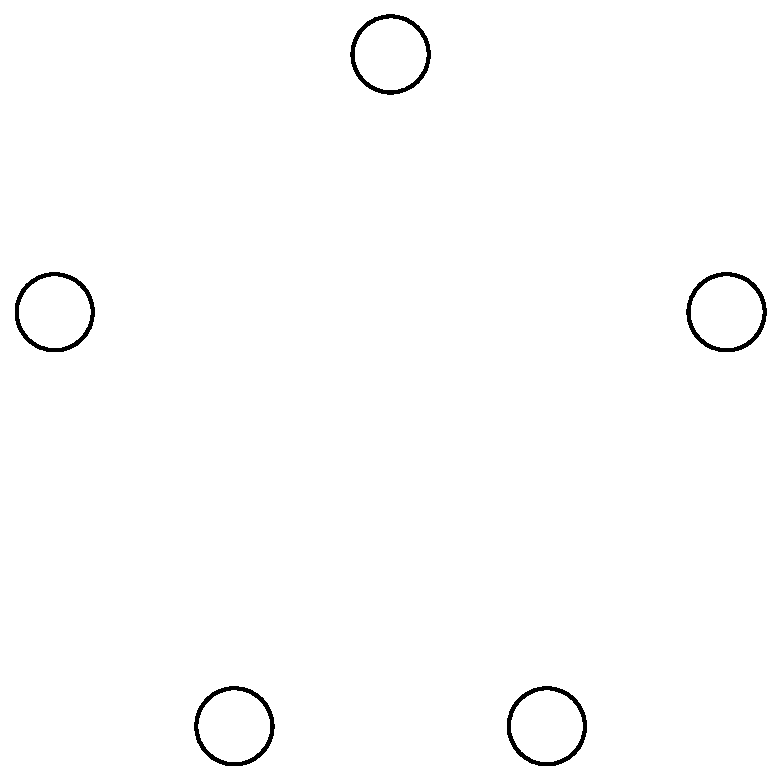
\includegraphics[scale=.25]{5.pdf}}\hspace{1in}\pause
			\subfloat{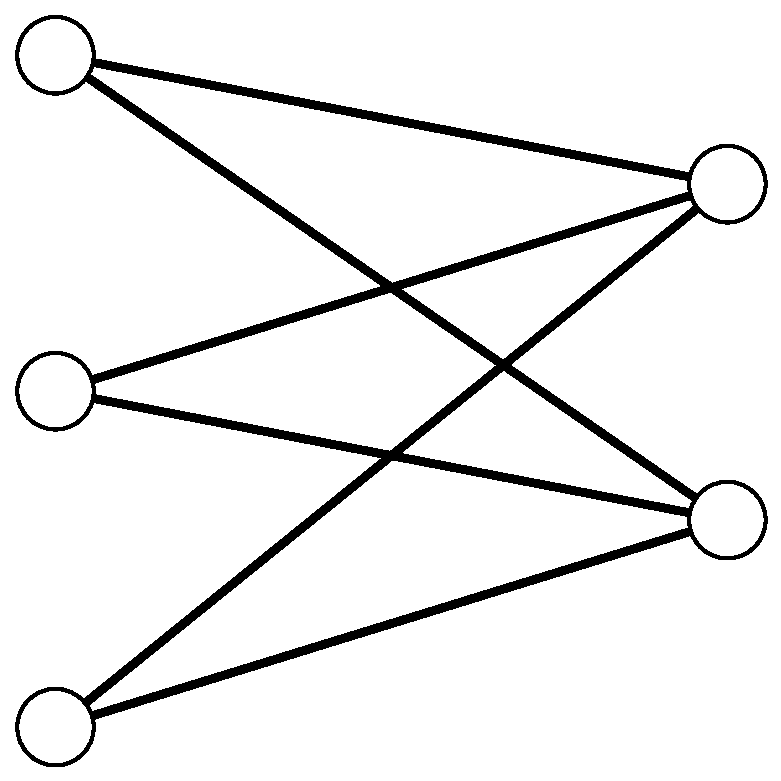
\includegraphics[scale=.25]{K_32.pdf}}
		\end{figure}	
	\end{frame}


	\begin{frame}{Guaranteeing the existence of a subgraph}
		\begin{itemize}

			\begin{theorem}[W. Mantel - 1907]
				If $G$ is a graph on $n$ vertices with more than $\lfloor n/2\rfloor \lceil n/2 \rceil$ edges, then $G$ contains a triangle.
			\end{theorem}

			\pause

			\item The graph on $n$ vertices with all possible edges is called the \textbf{complete graph} and is denoted $K_n$.

			\pause

			\begin{theorem}[P. Tur\'an - 1941]
				If $G$ is a graph on $n$ vertices with more than $(1-\frac{1}{r})\frac{n^2}{2}$ edges, then $G$ contains a copy of $K_{r+1}$.
			\end{theorem}
		\end{itemize}
	\end{frame}


	\begin{frame}{What about other graphs?}
		\begin{itemize}
			\item Given a graph $H$, the \textbf{extremal number} (or \textbf{Tur\'an number}) $\text{ex}(n, H)$ is the largest number of edges in an $H$-free graph on $n$ vertices.

			\pause

			\begin{theorem}[P. Erd\H{os}, A. Stone - 1946]
				Let $H$ be a nonempty graph and let $r$ be the \textbf{chromatic number} of $H$ (the smallest number of colors needed to color the vertices of $H$ so that no two adjacent vertices are of the same color). Then
				\[
					\text{ex}(n, H) = \left(1-\frac{1}{r-1}\right)\binom{n}{2} + o(n^2).
				\]
			\end{theorem}

			% \pause

			% \item Problems related to embedding subgraphs based on the number of edges in the host graph are called \textbf{Tur\'an-type problems}.
		\end{itemize}
	\end{frame}


	\begin{frame}{What about other graphs?}
		\begin{itemize}
			\item Apparently, the case of a \textbf{bipartite graph} (one whose chromatic number is 2) is exceptional.
			We only know the correct order of magnitude for such graphs in specific cases.

			\pause

			\item If $T$ is a \textbf{tree} (a graph which contains no cycles), then $\text{ex}(n, T) = \Theta(n)$.

			\pause

			\item Erd\H{os} showed that $\text{ex}(n, C_{2k})  = O(n^{1 + 1/k})$ for even cycles $C_{2k}$.
			Matching lower bounds are only known for $C_4$, $C_6$ and $C_{10}$.

			\pause

			\item Problems related to embedding subgraphs based on the number of edges in the host graph are called \textbf{Tur\'an-type problems}.
		\end{itemize}
	\end{frame}


	\begin{frame}{Larger substructures}
		\begin{itemize}
			\item Suppose we have 16 sports teams.
			Due to travel restrictions, some teams cannot play each other.
			How many pairs of teams that can play each other do we need to ensure that we can pair off all teams?

			\pause

			\item If even one team is unable to play with all the other teams, it can't be done.

			\pause

			\item Say we have a network of cities and roads between them.
			We have important deliveries to make in each city and we need to come back to where we started at the end of the day.
			How many roads do we need to guarantee that we need to visit each city only once?

			\pause

			\item We can't do this if there's only one road into any particular city.
		\end{itemize}
	\end{frame}


	\begin{frame}{Larger substructures}
		\begin{definition}
			Let $G = (V, E)$ be a graph.
			A subset of edges $\mathcal{M}\subseteq E$ is called a \textbf{matching} if its edges are vertex-disjoint.
			The matching $\mathcal{M}$ is \textbf{perfect} if the vertices that comprise it cover all of $V$.
		\end{definition}

		\pause

		\begin{definition}
			Let $G = (V, E)$ be a graph and let $\mathcal{C}$ be a sequence of edges.
			Then $\mathcal{C}$ is a \textbf{Hamiltonian cycle} if it is a cycle that visits every vertex in $G$ exactly once.
		\end{definition}

		% \begin{definition}
		% 	Let $G = (V, E)$ be a graph and let $\mathcal{C}$ be a sequence of edges.
		% 	Then $\mathcal{C}$ is a...
		% 	\begin{itemize}
		% 		\item ...\textbf{path} if it joins a sequence of distinct vertices.
		% 		\pause
		% 		\item ...\textbf{cycle} if it joins a sequence of vertices $v_1, v_2, \ldots, v_k, v_1$, where the internal vertices are distinct.
		% 		\pause
		% 		\item ...\textbf{Hamiltonian cycle} if it is a cycle that visits every vertex in $G$ exactly once.
		% 	\end{itemize}
		% \end{definition}
	\end{frame}


	\begin{frame}{Larger substructures}
		\begin{figure}
			\begin{overprint}
				\onslide<1>\centering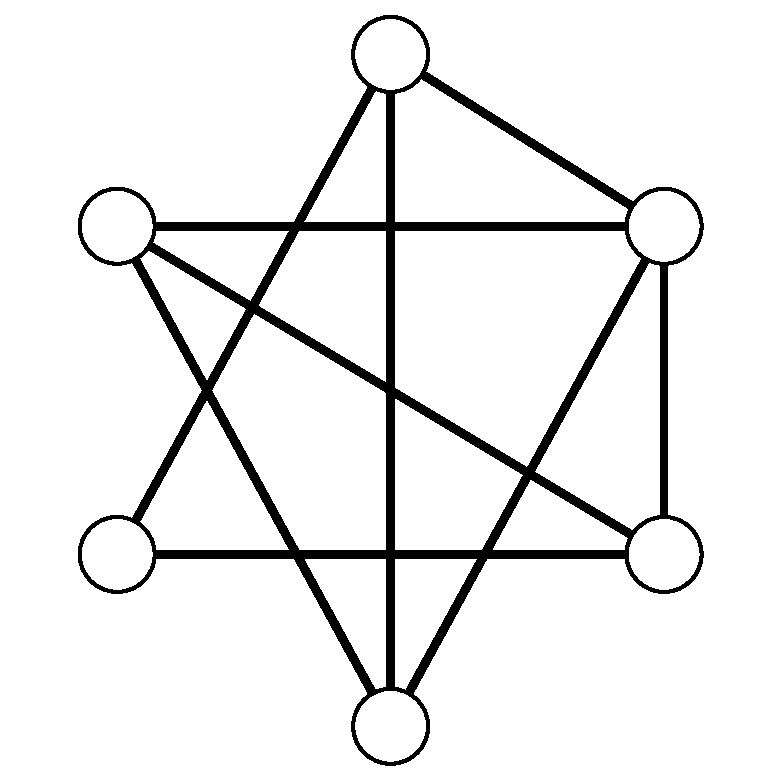
\includegraphics[scale=.5]{6.pdf}\caption{A graph}
				\onslide<2>\centering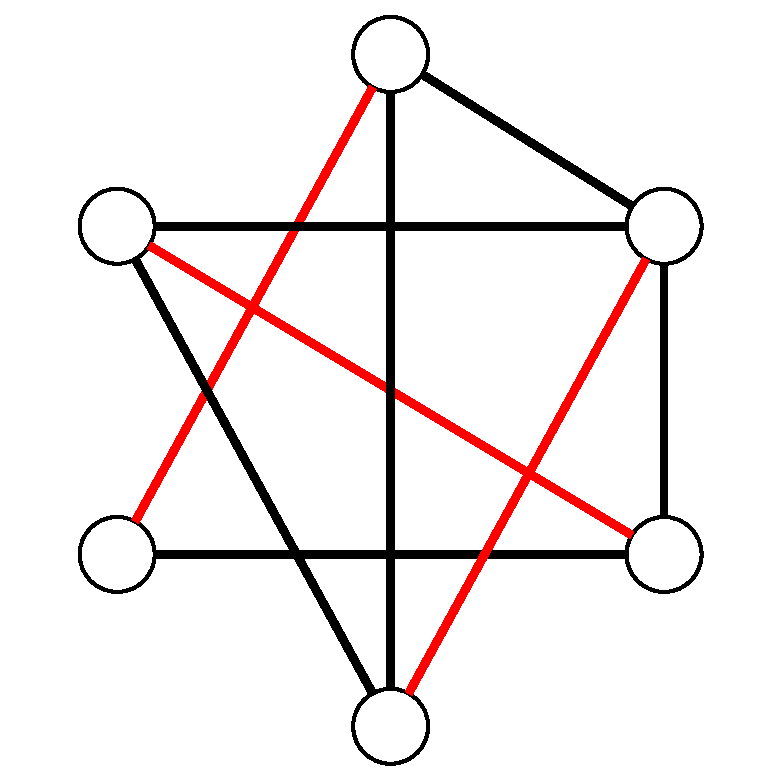
\includegraphics[scale=.5]{matching.pdf}\caption{A perfect matching}
				\onslide<3>\centering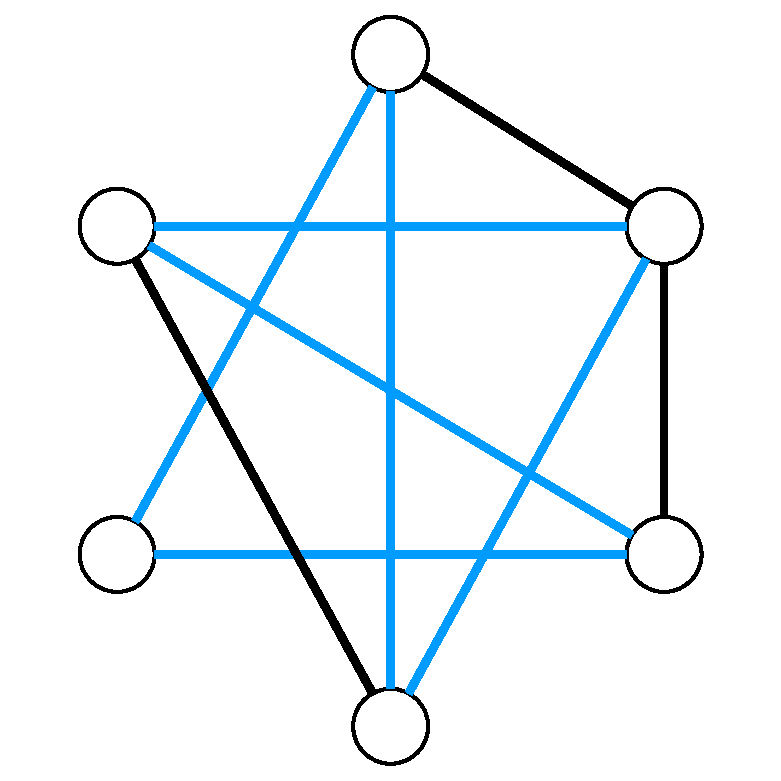
\includegraphics[scale=.5]{ham_cycle.pdf}\caption{A Hamiltonian cycle}
			\end{overprint}
		\end{figure}
	\end{frame}


	\begin{frame}{Another perspective}
		\begin{itemize}

			\item How many edges do we need to force a perfect matching or Hamiltonian cycle?

			\pause

			\item This question is a bit different from asking about $\text{ex}(n, H)$ for some $H$ since now our subgraph isn't fixed - it depends on $n$.

			\pause

			\item The Tur\'an perspective doesn't tell us much about perfect matchings - start with $K_n$ and delete all edges incident to one fixed vertex.
			The resulting graph has no perfect matching.

			\pause

			\begin{theorem}[P. Hall - 1935]
				Let $G$ be a bipartite graph with parts $X$ and $Y$ (all edges in $G$ have one end in $X$ and one end in $Y$).
				Then $G$ contains a matching that saturates $X$ if and only if every subset $W$ of $X$ has at least $|W|$ neighbors in $Y$.
			\end{theorem}	

		\end{itemize}
	\end{frame}

	\begin{frame}{Another perspective}
		\begin{itemize}
			\item Similarly, if any vertex has degree less than 2, we cannot have a Hamiltonian cycle.

			\pause

			\begin{theorem}[G. Dirac - 1952]
				A graph on $n\geq 3$ vertices contains a Hamiltonian cycle if $\delta(G)\geq n/2$ (graphs with such minimum degree are called \textbf{Dirac graphs}). In particular, such a graph contains a perfect matching if $n$ is even.
			\end{theorem}

			\pause

			\item Apparently, some structures aren't simply related to the number of edges in the host graph, but how they're distributed.
			
			\pause
			
			\item Graph embedding problems relating to the degree of the host graph are called \textbf{Dirac-type problems}.
		\end{itemize}
	\end{frame}



















\section{Counting perfect matchings and Hamiltonian cycles}
	

	\begin{frame}{From one to many}
		\begin{itemize}
			\item If a graph has sufficiently high minimum degree, it contains a Hamiltonian cycle (and a perfect matching if there is an even number of vertices).
			Could it have many?

			\pause

			\item The \textbf{Erd\H{o}s-Renyi random graph}, $\mathcal{G}(n, p)$, is the random variable that outputs a graph on $n$ vertices, any two of which are independently connected with probability $p$.
			It's one of the most well-studied random structures.

			% \pause
			
			% \item Say we're interested in some graph property, e.g. "has a Hamiltonian cycle."
			% Does there exist some value of $p$ for which $G\sim \mathcal{G}(n, p)$ has this property with high probability (whp)?

			% \pause

			% \item A function $r(n)$ is a \textbf{threshold function} for some property $P$ if whenever $p = o(r(n))$, $G\sim \mathcal{G}(n, p)$ does not satisfy $P$ whp, and whenever $p = \omega(r(n))$, $G$ satisfies $P$ whp.


			% \item If $G\sim \mathcal{G}(n, p)$, then 
			% \begin{align*}
			% 	\E[\#\{\text{perfect matchings in }G\}] &= \frac{n!}{2^{n/2}(n/2)!}p^{n/2},\\
			% 	\E[\#\{\text{Hamiltonian cycles in }G\}] &= \frac{1}{2}(n-1)!p^n.
			% \end{align*}
		\end{itemize}
	\end{frame}


	% \begin{frame}{Random graphs}
	% 	\begin{itemize}
	% 		\begin{theorem}[B. Bollob\'as, A. Thomason - 1987]
	% 			If $P$ is a monotone property (adding edges doesn't violate it), then $P$ has a threshold function (e.g. $\frac{\log n}{n}$ for connectivity and $\frac{\log n + \log\log n}{n}$ for Hamiltonicity). 
	% 		\end{theorem}

	% 		\pause

	% 		\item Random Tur\'an-like questions: threshold for containing some graph $H$ as a subgraph?
	% 		``Contains $H$'' is a monotone property.

	% 		\pause

	% 		\item Example: $G\sim \mathcal{G}(n, p)$ contains a triangle whp if $p = \frac{d}{n}$ for $d > \sqrt[3]{6}$ and it doesn't if $d<\sqrt[3]{6}$.

	% 	\end{itemize}
	% \end{frame}


	\begin{frame}{From one to many - intuition from random graphs}
		\begin{itemize}
			\item Idea: if $p>1/2$, then $G\sim \mathcal{G}(n,p)$ is Dirac whp.
			Maybe we can use probabilistic tools to estimate the number of perfect matchings/Hamiltonian cycles in $G$.
			Does this tell us anything about deterministic Dirac graphs?

			\pause

			\item Expected number of perfect matchings ($n$ even): $\frac{n!}{2^{n/2}(n/2)!}p^{n/2}$.

			\pause

			\item Expected number of Hamiltonian cycles: $\frac{1}{2}(n-1)!p^n$.

			\pause

			\item By Markov's inequality, $G\sim \mathcal{G}(n,p)$ doesn't have ``too many'' Hamiltonian cycles (perfect matchings) whp.

			\pause

			\item Glebov and Krivelevich showed that if $p = \frac{\log n + \log \log n + \omega(1)}{n}$, then the number of Hamiltonian cycles in $G\sim \mathcal{G}(n,p)$, up to a sub-exponential factor, concentrates about its mean.



			% \pause

			% \item Dirac graphs contain, up to a subexponential factor, at least as many Hamiltonian cycles (perfect matchings) as one would expect from the random graph.
		\end{itemize}	
	\end{frame}


	\begin{frame}{From one to many - intuition from random graphs}
		\begin{itemize}
			\begin{theorem}[B. Cuckler, J. Kahn - 2009]
				If $G$ is a graph on $n$ vertices with $\delta(G) \geq n/2$, then
				\begin{align*}
					\#\{\text{perfect matchings in }G\} &\geq (1-o(1))^n\cdot \frac{n!}{2^n(n/2)!}\\
					\#\{\text{Hamiltonian cycles in }G\} &\geq (1-o(1))^n\cdot \frac{1}{2^n}(n-1)!
				\end{align*}
			\end{theorem}

			\pause

			\item Edge disjoint cycles? Covering? Directed graphs?

		\end{itemize}	
	\end{frame}


	\begin{frame}{A riddle}
		\begin{itemize}
			\begin{problem}[T. Kirkman - 1850] %Lady's and Gentleman's Diary
				Fifteen young ladies in a school walk out three abreast seven days in succession: it is required to arrange them daily so that no two shall walk twice abreast.
			\end{problem}

			\pause

			\item Consider the set of ladies $H$ and let $E$ be the collection of subsets of $H$ of the form $\{\ell_1, \ell_2, \ell_3\}$, where the ladies $\ell_1$, $\ell_2$ and $\ell_3$ walk together on some day.

			\pause

			\item Sounds like a graph, except edges are triples!

			\pause 

			\item Kirkman's problem is asking us to find something resembling a collection of perfect matchings.
		\end{itemize}
	\end{frame}


	\begin{frame}{A generalization - hypergraphs}
		\begin{itemize}
			\item A \textbf{hypergraph} $H = (V, E)$ consists of a set of vertices $V$ and a set of edges $E\subseteq 2^V$.
			We say that $H$ is $k$-uniform if every edge consists of exactly $k$ vertices (note that a graph is a 2-uniform hypergraph).

			\pause

			\item We can talk about Tur\'an or Dirac-type problems in this setting too.

			\pause

			\item More generalized notion of degree: if $S$ is any subset, then $d(S)$ is the number of edges that contain $S$.
			$\delta_t(H)$ is the minimum of $d(S)$ over all subsets of size $t$.
		\end{itemize}
	\end{frame}


	\begin{frame}{Generalizing the substructures}
		\begin{itemize}
			\item Can we extend the notions of matchings and cycles to hypergraphs?

			\pause

			\item Matchings seem fine.

			\pause

			\item Cycles are a bit less clear since the edges in graph cycles overlap at the ends.
			How can we account for this in hypergraphs?

			\pause

			\item We say that a $k$-uniform hypergraph $H$ contains a \textbf{Hamiltonian $\ell$-cycle} if there is a cyclic ordering of the vertices of $H$ such that the edges of the cycle are segments of length $k$ in this ordering and any two consecutive edges $f_i$, $f_{i+1}$ share exactly $\ell$ vertices.
		\end{itemize}
	\end{frame}


	\begin{frame}{Example}
		\begin{figure}
			\begin{overprint}
				\onslide<1>\centering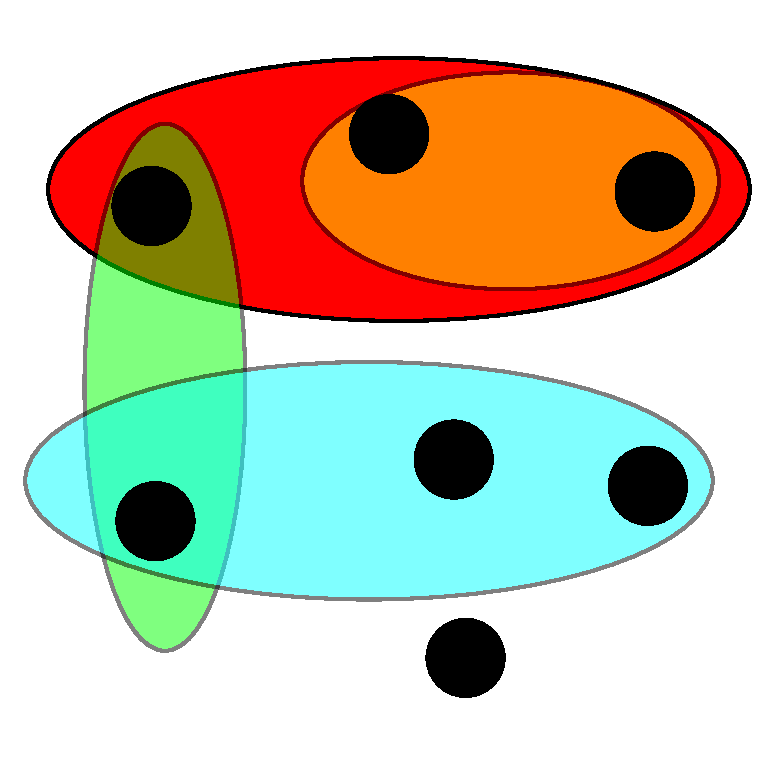
\includegraphics[scale=.5]{hyper.pdf}\caption{A hypergraph}
				\onslide<2>\centering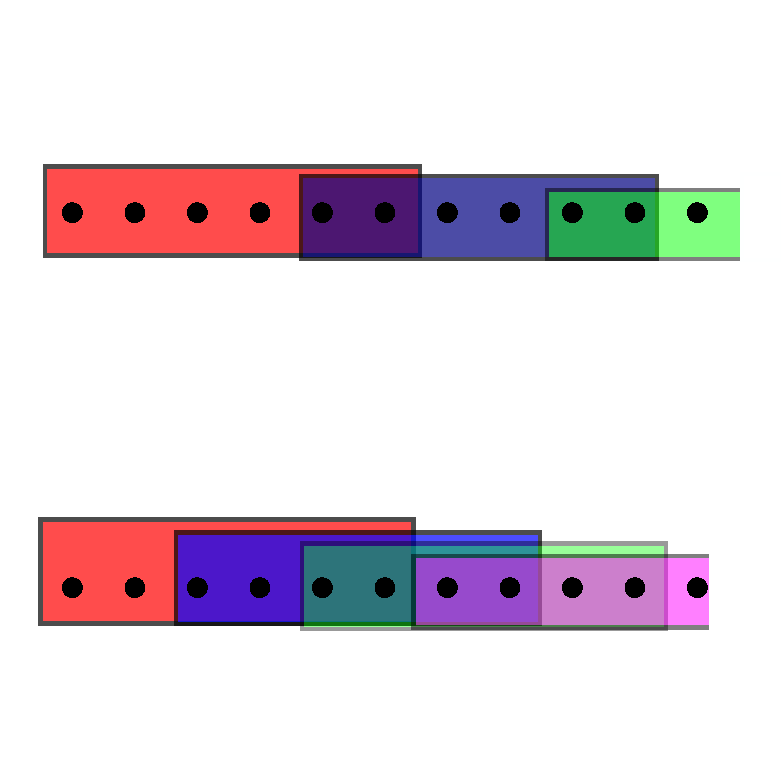
\includegraphics[scale=.5]{hyper_cycles.pdf}\caption{Top: $k = 6$, $\ell = 2$.\quad Bottom: $k = 6$, $\ell = 4$.}
			\end{overprint}
		\end{figure}
	\end{frame}


	\begin{frame}{Matchings and cycles in hypergraphs}
		\begin{itemize}
			\item Notice that if $\ell = 0$, then a Hamiltonian $\ell$-cycle is a perfect matching.

			\pause 
			
			\item If $\ell > k/2$, \emph{three} consecutive edges in an $\ell$-cycle overlap.
			This ostensibly makes counting these more nuanced.

			\pause

			\item For $\ell \leq k/2$, the number of Hamiltonian $\ell$-cycles we expect to see in a random hypergraph with edge probability $p$ is
			\[
				(n-1)!\cdot \frac{k-\ell}{2}\cdot \left(\frac{p}{\ell!(k-2\ell)!}\right)^{\frac{n}{k-\ell}}.
			\]

		\end{itemize}
	\end{frame}
	
	\begin{frame}{Matchings and cycles in hypergraphs}
	    \begin{itemize}
    		\begin{theorem}[A. Ferber, M. Krivelevich, B. Sudakov - 2016]
    			Let $0\leq \ell < k/2$ and let $1/2 < p \leq 1$.
    			If $(k-\ell)\mid n$ and $\delta_{k-1} \geq pn$, then the number of Hamiltonian $\ell$-cycles in the $k$-uniform hypergraph $H$ is at least
    			\[
    			(1-o(1))^n\cdot n!\cdot \left(\frac{p}{\ell!(k-2\ell)!}\right)^{\frac{n}{k-\ell}}.
    			\]
    		\end{theorem}
    		
    		\pause
    		
    		%\item Notice that we had to change the notion of vertex degree in the hypergraph version of the theorem.
    		%Given a $(k-1)$ subset $X$ in a $k$-graph, the number of edges that contain $X$ is called its \textbf{co-degree}, $d_{k-1}(X)$.
    		%Similarly, the minimum co-degree of a $k$-graph $H$ is denoted $\delta_{k-1}(H)$.

    		\item Notice that the minimum \textbf{co-degree}, $\delta_{k-1}(H)$ plays a role analogous to the minimum degree in a graph.
    		A \textbf{Dirac hypergraph} on $n$ vertices is one whose minimum co-degree is at least $n/2$.
		\end{itemize}
	\end{frame}


	\begin{frame}{Matchings and cycles in hypergraphs - current work}
		\begin{itemize}
			% \begin{theorem}[A. Ferber, H., A. Mond - 2020+]
			% 	Let $0\leq \ell < k-1$ and let $1/2 < p \leq 1$.
			% 	If $(k-\ell)\mid n$ and $\delta_{k-1}(H) \geq pn$, then the number of Hamiltonian $\ell$-cycles in $H$ is at least
			% 	\[
			% 	(1-o(1))^n\cdot n!\cdoot \left(\frac{p}{})
			% 	\]
			% \end{theorem}

			\item Extending the work of Ferber, Krivelevich and Sudakov to the case $\ell < k-1$.
			Joint with A. Mond (University of Cambridge)

			\pause

			\item Future work: a tight (up to subexponential factor) bound for tight ($\ell = k-1$) cycles; number of \emph{disjoint} $\ell$-cycles.
		\end{itemize}
	\end{frame}





















\section{Degrees of prescribed remainder}

	\begin{frame}{A motivating problem}
		\begin{itemize}
			% \begin{exercise}[L. Lov\'asz, T. Gallai - 1979]
			% 	(Stated as an exercise in Lov\'asz' book).
			% 	Let $G = (V, E)$ be any graph.
			% 	Then $G$ admits a partitioning of its vertex set into two parts, $V = V_1 \cup V_2$, so that each vertex in $G[V_1]$ and each vertex in $G[V_2]$ has even degree.
			% 	In particular, any graph on $n$ vertices has an even subgraph of order at least $n/2$.
			% \end{exercise}\pause
			\begin{exercise}[L. Lov\'asz, T. Gallai - 1979]
				Assume that at each vertex of a graph there is a light that is turned on.
				Toggling any light toggles all of its neighbors as well.
				Turn off all of the lights.
			\end{exercise}\pause


			\item Solution: find some $X\subseteq V(G)$ where all degrees in $G[X]$ are even and every $v\notin X$ has odd degree into $X$.
			Then toggle every light in $X$.

			\pause

			\item Every light in $V\setminus X$ flips an odd number of times (each of its neighbors in $X$) and every light in $X$ flips an odd number of times (each of its neighbors in $X$ and itself).


		\end{itemize}	
	\end{frame}


	\begin{frame}{Even degrees}
		\begin{itemize}
			\begin{theorem}[L. Lov\'asz, T. Gallai - 1979]
				(Stated as an exercise in Lov\'asz' book).
				Let $G = (V, E)$ be any graph.
				Then $G$ admits a partitioning of its vertex set into two parts, $V = V_1 \cup V_2$, so that each vertex in $G[V_1]$ and each vertex in $G[V_2]$ has even degree.
				In particular, any graph on $n$ vertices has an even subgraph of order at least $n/2$.
			\end{theorem}

			\pause

			\item Use this theorem to prove that our solution is possible.

			\pause

			\item This theorem contains two statements: one about a large induced subgraph and another about partitioning into particular subgraphs.
		\end{itemize}
	\end{frame}


	\begin{frame}{Odd subgraphs}
		\begin{itemize}
			\item What about odd subgraphs?\pause

			\begin{theorem}[A. Scott - 1992]
				Every graph $G(V, E)$ on $n$ vertices, none of which are isolated, contains a set $W\subseteq V(G)$ such that $|W|\geq \frac{n}{900 \log n}$ and $G[W]$ has all degrees odd.
			\end{theorem}\pause

			\begin{conjecture}[A. Scott - 2001]
				There exists some constant $c>0$ such that every graph $G(V, E)$ on $n$ vertices, none of which are isolated, contains a set $W\subseteq V(G)$ such that $|W|\geq cn$ and $G[W]$ has all degrees odd.
			\end{conjecture}
		\end{itemize}
	\end{frame}


	\begin{frame}{Other moduli and remainders}

		\begin{theorem}[A. Scott - 1992]
			Let $G\sim \mathcal{G}(n, 1/2)$.
			Then with high probability, $G$ has an induced subgraph on at least $0.7729n$ vertices with all degrees odd.
		\end{theorem}\pause

		\begin{conjecture}[A. Scott - 2001]
			For any positive integer $q$ at least 2, there exists a constant $c_q$ so that every graph on $n$ vertices without isolated vertices has an induced subgraph on at least $c_qn$ vertices with all degrees $1\pmod q$.
		\end{conjecture}
	\end{frame}


	\begin{frame}{Other moduli and Remainders}
		% \begin{definition}
		% 	Let $q$ be a positive integer at least 2 and let $0\leq r<q$ be an integer.
		% 	If $G$ is a graph, we write $f(G, r, q)$ for the maximum order of an induced subgraph of $G$ with all degrees $r\pmod q$.
		% \end{definition}
		\begin{theorem}[A. Ferber, H., M. Krivelevich - 2020+]
			Let $q\geq 2$ and let $r$ be an integer.
			Then there exists a constant $c_q$ such that, with high probability, the random graph $G\sim \mathcal{G}(n, 1/2)$ has an induced subgraph on at least $c_qn$ vertices with all degrees $r\pmod q$.
		\end{theorem}
	\end{frame}


	\begin{frame}{Key idea behind proof}
		\begin{itemize}
			\item If $G\sim \mathcal{G}(n, 1/2)$, then its adjacency matrix $M$ ($M_{ij} = 1$ if and only vertices $i$ and $j$ are connected and $M_{ij}=0$ otherwise) is a random symmetric $n\times n$ matrix whose above-diagonal entries are iid $\Bern(1/2)$ random variables.

			\pause

			\item In this case, the $i$-th entry of $M\boldsymbol{1}$ is the degree of vertex $i$ in $G$, where $\boldsymbol{1}$ is the length $n$ all-1 vector.

			\pause

			\begin{observation}
				$G$ contains an induced subgraph with all degrees $r\pmod q$ if and only if its adjacency matrix contains a principal submatrix $B$ satisfying $B\boldsymbol{1} \equiv r\boldsymbol{1}\pmod q$.
			\end{observation}
		\end{itemize}
	\end{frame}


	\begin{frame}{Proof (sketch) of theorem}
		\begin{itemize}
			\begin{theorem}[Chebyshev's Inequality]
				Let $X$ be a nonnegative integer-valued random variable with finite variance.
				Then
				\[
					\Pr[X > 0] \geq 1 - \frac{\Var[X]}{(\E[X])^2}.
				\]

			\end{theorem}

			\pause

			\item Let $k = c_qn$ for some $c_q>0$ and let $X_k$ be the number of $k\times k$ principal submatrices $B$ of the adjacency matrix of $G$ satisfying $B\boldsymbol{1} \equiv r\boldsymbol{1} \pmod {q}$.

			\pause

			\item Show that $c_q$ can be chosen so that $\Var[X_k] = o(E[X_k]^2)$.
			Then $G$ has an induced subgraph of size $c_qn$ with high probability.
		\end{itemize}
	\end{frame}


	\begin{frame}{Key computation}
		Fix a positive integer $q\geq 2$ and let $r$ be an integer.
		Let $x_1, \ldots, x_t$ be iid $\Bern(1/2)$ random variables. If $\delta_0(x) = 1$ if and only if $x \equiv 0\pmod q$ and $\delta_0(x) = 0$ otherwise, then

		\pause

		\begin{align*}
			\Pr[x_1 + \cdots + x_t \equiv r] &= \E[\delta_0(x_1 + \cdots + x_t - r)]\\
			\uncover<3->{&= \frac{1}{q}\sum_{\ell\in \Z_q}\E\exp\left[\frac{2\pi i\ell}{q}(x_1 + \cdots  + x_t - r) \right]\\}
			\uncover<4->{&=\frac{1}{q}\sum_{\ell\in \Z_q}e^{-2\pi ir \ell/q}\prod_{j=1}^t\E e^{2\pi i \ell x_j/q}\\}
			\uncover<5->{&= \frac{1}{q}\sum_{\ell\in \Z_q}e^{-2\pi ir \ell/q}\left(\frac{1+e^{2\pi i\ell/q}}{2}\right)^t.}
		\end{align*}
	\end{frame}


	\begin{frame}{Key computation}
		\begin{itemize}
			\item Isolate the $\ell \equiv 0$ term, apply the triangle inequality and Euler's identity.

			\pause

			\begin{align*}
				\left|\Pr[x_1 + \cdots + x_t \equiv r] - \frac{1}{q}\right|\leq \frac{1}{q}\sum_{\ell = 1}^{q-1}|\cos(\pi \ell/q)|^t.
			\end{align*}

			\pause

			\item Calculus trick: $|\cos(\pi \ell/q)|\leq e^{-2/q^2}$ for all $\ell = 1, \ldots, q-1$.

			\pause

			\[
				\left|\Pr[x_1 + \cdots + x_t \equiv r] - \frac{1}{q}\right|\leq \frac{q-1}{q}e^{-2t/q^2}.
			\]
		\end{itemize}
	\end{frame}


	\begin{frame}{Key computation}
		\begin{itemize}
			\item The distribution of a random Bernoulli sum modulo $q$ is asymptotically uniform!

			\pause

			\item Using this, we can show that if $M$ is the adjacency matrix of a random graph, then $M\boldsymbol{1} \pmod q$ is (asymptotically) distributed uniformly over all possible values it can take.


			% \begin{lemma}
			% 	Let $M$ be an $s\times t$ matrix whose entries are iid $\Bern(1/2)$ random variables.
			% 	Then for any $v\in \Z_q^s$,
			% 	\[
			% 		%\Pr[M\boldsymbol{1} \equiv v] = \frac{1}{q^s}\bigg(1 + O\left(e^{-2t/q^2}\right)\bigg)^s.
			% 		\Pr[M\boldsymbol{1} \equiv v] = \frac{1}{q^s}(1+o_t(1))^s
			% 	\]
			% \end{lemma}	
		\end{itemize}
	\end{frame}


	% \begin{frame}{Symmetric case}
	% 	\begin{itemize}
	% 		\item But the adjacency matrix is symmetric!

	% 		\pause

	% 		% \item A similar, but more technical argument handles the symmetric case.

	% 		% \pause

	% 		\begin{lemma}
	% 			Let $M$ be an $m\times m$ symmetric matrix whose diagonal is zero and whose entries above the diagonal are iid $\Bern(1/2)$ random variables.
	% 			Then for any $v\in \Z_q^m$,
	% 			\[
	% 				% \Pr[M\boldsymbol{1} \equiv v] = \begin{cases}
	% 				% 	\frac{1}{q^m}(1 + O(e^{-m/q^2})) & \text{ if $q$ is odd}\\
	% 				% 	\frac{2}{q^m}(1 + O(e^{-m/q^2})) & \text{ if $q$ is even and $\sum v_i$ is even}\\
	% 				% 	0 & \text{ if $q$ is even and $\sum v_i$ is odd}.
	% 				% \end{cases}
	% 				\Pr[M\boldsymbol{1} \equiv v] = \begin{cases}
	% 					\frac{1}{q^m}(1 +o(1)) & \text{ if $q$ is odd}\\
	% 					\frac{2}{q^m}(1 + o(1)) & \text{ if $q$ is even and $\sum v_i$ is even}\\
	% 					0 & \text{ if $q$ is even and $\sum v_i$ is odd}.
	% 				\end{cases}
	% 			\]
	% 		\end{lemma}
	% 	\end{itemize}
	% \end{frame}


	% \begin{frame}{Parity?}
	% 	\begin{itemize}
	% 		\item We have
	% 		\[
	% 			\sum_i (M\boldsymbol{1})_i = \sum_{i,j} M_{ij} = 2\sum_{i<j}M_{ij},
	% 		\]
	% 		which is always even modulo $q$ if $q$ is even and can be any residue modulo odd $q$.

	% 		\pause

	% 		\item The symmetric lemma then says that the distribution of $M\boldsymbol{1}\pmod q$ is asymptotically uniform over all ``feasible'' values.
	% 	\end{itemize}
	% \end{frame}


	\begin{frame}{Partitioning}
			\begin{theorem}[L. Lov\'asz, T. Gallai - 1979]
				Let $G = (V, E)$ be any graph.
				Then $G$ admits a partitioning of its vertex set into two parts, $V = V_1 \cup V_2$, so that each vertex in $G[V_1]$ and each vertex in $G[V_2]$ has even degree.
				In particular, any graph on $n$ vertices has an even subgraph of order at least $n/2$.
			\end{theorem}\pause

			\begin{theorem}[A. Ferber, H., M. Krivelevich, 2020+]
				For $q>1$ and $r\leq q$, $G\sim \mathcal{G}(n, 1/2)$ admits a partition into $q+1$ classes such that the degrees in each class are congruent to $r\pmod q$ with high probability.
			\end{theorem}

	\end{frame}


	% \begin{frame}{Packing theorems}
	% 	\begin{theorem}[A. Scott - 2001]
	% 		Let $G$ be a graph. Then $G$ admits a partition into odd subgraphs if and only if every component of $G$ has even order.
	% 	\end{theorem}

	% 	\pause

	% 	\begin{theorem}[A. Scott - 2001]
	% 		With high probability, $G\sim \mathcal{G}(n, p)$ for $n$ even admits a partition into three odd subgraphs.
	% 	\end{theorem}

	% 	\pause

	% 	\begin{conjecture}[A. Scott - 2001]
	% 		For $q>1$ and $r \leq q$, there exists a constant $c_q$ such that $G\sim \mathcal{G}(n, p)$ admits a partition into $c_q$ classes such that the degrees in each class are congruent to $r\pmod q$ with high probability.
	% 	\end{conjecture}
	% \end{frame}


	% \begin{frame}{Packing theorems}
	% 	\begin{itemize}
	% 		\begin{theorem}[A. Ferber, H., M. Krivelevich, 2020+]
	% 			For $q>1$ and $r\leq q$, $G\sim \mathcal{G}(n, 1/2)$ admits a partition into $q+1$ classes such that the degrees in each class are congruent to $r\pmod q$ with high probability.
	% 		\end{theorem}

	% 		\pause

	% 		\item The proof is another second moment argument.
	% 	\end{itemize}
	% \end{frame}


	\begin{frame}{Future work - discrete Fourier analysis}
		% \begin{itemize}
		% 	\item Other applications of disc
		% \end{itemize}

		\begin{theorem}[A. Ferber - 2020]
			Let $M_n$ denote an $n\times n$ symmetric $\pm 1$ matrix chosen uniformly from all such matrices.
			Let $p(n)$ denote the probability that $M_n$ is singular.
			Then there exists some constant $C>0$ for which
			\[
				p(n) = O\left(\frac{\log^Cn}{\sqrt{n}}\right).
			\]
		\end{theorem}
	\end{frame}


	\begin{frame}{Future work - discrete Fourier analysis}
		\begin{theorem}[R. Meshulam - 1990]
			Let $G$ be a finite abelian group and let $s(G)$ denote the maximal $s$ for which there exists a sequence $a_1, \ldots, a_s\in G$ such that $\sum_{i\in I}a_i \neq 0$ for any nonempty $I\subseteq [s]$.
			Then if $m$ is the maximum order of elements in $G$, we have
			\[
				s(G)\leq m\left(1 + \log\frac{|G|}{m}\right).
			\]
		\end{theorem}	
	\end{frame}


	\begin{frame}{Future work - discrete Fourier analysis}
		\begin{itemize}
			\begin{conjecture}[N. Alon, N. Linial, R. Meshulam - 1988]
				For every prime $p$, there exists a constant $c_p$ such that for any $n\geq 1$, the union of any $c_p$ linear bases for $\Z_p$ forms an additive basis for $\Z_p$.
			\end{conjecture}
			\pause

			\item The best known bound is at most $c_p \log n$ many linear bases.
		\end{itemize}
	\end{frame}


	\begin{frame}
		\centering\Large
		\emph{Thank you.}
	\end{frame}












%\section{Future work}








% \section{TODO}
% 	\begin{frame}{TODO}
% 		\begin{itemize}
% 			\item wrap up with ending
% 			\item PICTURES
% 			\item more connective tissue in degree remainders section: it's just a bunch of theorem statements
% 			\item Flesh out current work section on cycle counting: we think we have a theorem, but we're in the process of verifying our proof/methods

% 			\item Section on future problems I'm interested in: more applications of discrete Fourier analysis; substructures in Latin squares and Steiner triple systems.
% 		\end{itemize}
% 	\end{frame}
\end{document}
